\chapter[Forschungsfrage 3]{Welche besonderen sicherheitstechnischen Aspekte muss ein solcher Prozess im Bereich der Versicherung erfüllen?} \label{ff3}
Dieses Kapitel beschreibt Grundlagen zur Sicherheit in der Informationstechnik. Die Grundlagen beschäftigen sich mit der ISO-Norm 27001, die eine vollständige Beschreibung enthält, wie Systeme gesichert werden können. Darauf aufbauend beschäftigt sich dieses Kapitel mit dem Kompendium des IT-Grundschutzes des \ac{BSI}, das mittels vorgefertigten Bausteinen eine praktische Anleitung zur Sicherung der IT-Systeme bietet. Außerdem wird der \ac{SVI}-Einkaufsprozess von \enquote{Open source} analysiert. Das Kapitel schließt mit einem Soll-Ist-Vergleich zwischen den Bausteinen des \ac{BSI} und der Umsetzung in der \ac{SVI} ab. Daraus resultiert das Teilergebnis der Forschungsfrage drei.
\par
Informations- und Kommunikationssysteme sind in der heutigen Gesellschaft von elementarer Bedeutung -- sie spielen eine immer größer werdende Rolle. Der Innovationsgrad in der Informationstechnik ist konstant hoch und deswegen sind folgende Bereiche ständiger Weiterentwicklung unterworfen: steigende Vernetzung der Bevölkerung, IT-Verbreitung und Durchdringung, Verschwinden der Netzgrenzen, kürzere Angriffszyklen auf wichtige Infrastruktur, höhere Interaktivität von Anwendungen und die Verantwortung der Benutzer eines IT-Systems.\autocite[vgl.][S.\,2f.]{bundesamt_fur_sicherheit_in_der_informationstechnik_bsi_it-grundschutz-kompendium_2020}

\section{Grundlagen: sicherheitstechnische Anforderungen}\label{kap:sicherheitstechnischeAnforderungen}
Informationen sind elementarer Bestandteil der heutigen Welt und diese sind von sehr hohem Wert für Unternehmen, Behörden und Privatpersonen. Die meisten Geschäftsprozesse, die im heutigen Prozessablauf einer Organisation verankert sind, funktionieren nicht ohne IT-Unterstützung. Somit ist die Informationstechnologie zentraler Bestandteil jedes Unternehmens. Deswegen ist ein zuverlässiges System mit entsprechender Soft- und Hardware unerlässlich. Es muss darauf geachtet werden, dass die Informationen, die auf diesem System verteilt sind, ausreichend gut geschützt sind, damit es nicht zu einer Bedrohungslage kommt. Unzureichend geschützte Systeme stellen ein sehr hohes Risiko dar. \enquote{Dabei ist ein vernünftiger Informationsschutz ebenso wie eine Grundsicherung der IT schon mit verhältnismäßig geringen Mitteln zu erreichen. Die verarbeiteten Daten und Informationen müssen adäquat geschützt, Sicherheitsmaßnahmen sorgfältig geplant, umgesetzt und kontrolliert werden. Hierbei ist es aber wichtig, sich nicht nur auf die Sicherheit von IT-Systemen zu konzentrieren, da Informationssicherheit ganzheitlich betrachtet werden muss. Sie	hängt auch stark von infrastrukturellen, organisatorischen und personellen Rahmenbedingungen ab.}\autocite[][S.\,1]{bundesamt_fur_sicherheit_in_der_informationstechnik_bsi_it-grundschutz-kompendium_2020} Die Mängel in der IT-Sicherheit führen meist zu folgenden drei Kategorien von Problemen\autocite[vgl.][S.\,1ff.]{bundesamt_fur_sicherheit_in_der_informationstechnik_bsi_it-grundschutz-kompendium_2020}: 

\begin{itemize}
	\item Verlust der Verfügbarkeit
	\item Verlust der Vertraulichkeit
	\item Verlust der Integrität
\end{itemize}

Der Verlust der Verfügbarkeit eines IT-Systems fällt sofort auf, da meist Aufgaben ohne diese Informationen nicht weitergeführt werden können. Meist tritt dies in dem Verlust der Funktionen eines Systems zutage. Die Vertraulichkeit von personenbezogenen Daten ist ein bestehendes Grundrecht jedes Bürgers beziehungsweise jedes Kunden. Dies ist in verschiedenen Gesetzen wie auch Verordnungen geregelt. Diese Daten müssen geschützt werden, da jedes Konkurrenzunternehmen Interesse an den Daten des Unternehmens hat. \enquote{Gefälschte oder verfälschte Daten können beispielsweise zu Fehlbuchungen, falschen Lieferungen oder fehlerhaften Produkten führen. Auch der Verlust der Authentizität (Echtheit und Überprüfbarkeit) hat, als ein Teilbereich der Integrität, eine hohe Bedeutung: Daten werden beispielsweise einer falschen Person zugeordnet. So können Zahlungsanweisungen oder Bestellungen zulasten einer dritten Person verarbeitet werden, ungesicherte digitale Willenserklärungen können falschen Personen zugerechnet werden, die digitale Identität wird	gefälscht.}\autocite[][S.\,1]{bundesamt_fur_sicherheit_in_der_informationstechnik_bsi_it-grundschutz-kompendium_2020}

\paragraph{\ac{ISMS}}\label{kap:ISMS}
Um ein \ac{ISMS} besser verstehen zu können, ist es wichtig, die Normenreihe des ISO-27001-Standards zu kennen. So bietet die ISO-Norm 27000 einen Überblick über ein solches System und definiert Begrifflichkeiten. Die zentrale Norm ist die ISO 27001, die die \ac{ISMS}-Anforderungen beschreibt.\autocite[vgl.][]{dindeutsches_institut_fur_normung_informationstechnik_2020} Dieser Norm sind die ISO-Standards 27002-27005, ISO 27007 und ISO 27008 untergeordnet, welche verschiedene Detailfragen zu in ISO 27001 genannten Konzepten definieren. Die Normen entstanden im britischen Institut für Standards, weswegen \enquote{[...] [es] gleichzeitig eine international anerkannte Zertifizierungsstelle für ISO 27001 [ist] und damit eine der Stellen, die befugt sind, Auditoren zu qualifizieren und einzusetzen, um die Übereinstimmung einer Organisation mit der ISO 27001 im Rahmen einer Zertifizierung zu überprüfen.}\autocite[vgl.][S.\,2]{kersten_it-sicherheitsmanagement_2020} Die ISO-Norm 27001 ist durch die abstrakte Beschreibung und ihren Aufbau auf jegliche Art von Organisationen (Behörden, Unternehmen, Vereine, \ac{NGOs} u.\,Ä.) anwendbar. Außerdem ist sie beliebig skalierbar und in jedem Land bzw. länderübergreifend nutzbar.\autocite[vgl.][S.\,4]{kersten_it-sicherheitsmanagement_2020} Die ISO-Norm 27000 definiert: \enquote{Ein Informationssicherheitsmanagementsystem (ISMS) umfasst Politik, Verfahren, Richtlinien und damit verbundene Ressourcen und Tätigkeiten,   die alle von einer Organisation gesteuert werden, um ihre Informationswerte zu  schützen. Ein ISMS ist ein systematisches Modell für die Einführung, die Umsetzung,  den Betrieb, die Überwachung, die Überprüfung, die Pflege und die Verbesserung der Informationssicherheit einer Organisation, um Geschäftsziele zu erreichen.}\autocite[][S.\,20]{dindeutsches_institut_fur_normung_informationstechnik_2019}
\par
Die ISO-Norm 27001 definiert in Kapitel vier bis zehn Anforderungen an ein Management-System der Informationssicherheit.\autocite[vgl.][S.\,6-16]{dindeutsches_institut_fur_normung_informationstechnik_2020} \enquote{Als Management-System für ein Thema X bezeichnet man allgemein alles, was eingesetzt wird, um die wesentlichen Ziele für das Thema X zu ermitteln, diese Ziele zu erreichen und ihre Aufrechterhaltung zu überwachen.}\autocite[][S.\,5]{kersten_it-sicherheitsmanagement_2020} Nachfolgend sind die typischen Aktivitäten genannt\autocite[][S.\,5]{kersten_it-sicherheitsmanagement_2020}:
\begin{itemize}
	\item Ziele in Form von Leitlinien zu formulieren,
	\item Risiken und Chancen für diese Ziele zu analysieren,
	\item Rollen bzw. Verantwortlichkeiten für bestimmte (Teil-)Ziele zu definieren,
	\item Methoden oder Verfahren zu deren Erreichung zu vermitteln,
	\item den vom Thema X Betroffenen besondere Regelwerke oder Richtlinien aufzugeben,
	\item Prozesse bzw. Abläufe und dafür erforderliche Maßnahmen zu planen und umzusetzen,
	\item Überprüfungen der Zielerreichung zu planen, durchzuführen und auszuwerten.
\end{itemize}
Ziel des \ac{ISMS} und damit der ISO-Norm 27001 ist es, für möglichen Prozess/Aktivitäten der Informationssicherheit ein einheitliches, standardisiertes System zu gestalten. Damit werden Aufwand- und Kosteneinsparungen erzeugt und die Akzeptanz eines solchen Systems gesteigert. Beispielsweise implementiert die ISO-Norm 9001 ein Qualitätsmanagementsystem\autocite{dindeutsches_institut_fur_normung_qualitatsmanagementsysteme_2020}, wobei die Architekturen der beiden Systeme kompatibel sind. Das \ac{ISMS} wird auf die gesamte Organisation angewendet. Die wichtigsten Aufgaben sind dabei die Formulierung von Sicherheitszielen, die Bestimmung des \enquote{Assets}\footnote{\enquote{Unter Assets wird alles verstanden, was für eine Organisation einen Wert darstellt. Dies können zunächst Grundstücke, Gebäude, Maschinen und Anlagen, Geschäftsprozesse sein – aber natürlich auch die sogenannten Information Assets (Informationswerte) wie Informationen/Daten, Systeme, Anwendungen, IT Services. Ergänzend kann man auch Soft Assets betrachten wie das Image oder die Kreditwürdigkeit einer Organisation.} Quelle: \cite[][S.\,8]{kersten_it-sicherheitsmanagement_2020}.}, die Risikobeurteilung und -behandlung und die kontinuierliche Verbesserung. Die Sicherheitsziele beschreiben die in Kapitel \vref{kap:sicherheitstechnischeAnforderungen} genannten drei Hauptziele der Informationssicherheit (Verfügbarkeit, Vertraulichkeit und Integrität). Das Kapitel der Leitlinien beschäftigt sich mit der Definition der Organisation, der Analyse und den Regeln auf verschiedenen Ebenen der Organisation. Der Prozess der kontinuierlichen Verbesserung implementiert das Modell des \enquote{Plan-Do-Check-Act}-Regelkreises.\footnote{Eine Abbildung dieses ist im Anhang \vref{abb:planDoCheckAct} zu sehen.} Eine akzeptierte Variante ist, den Regelkreis jährlich zu durchlaufen. Umso mehr Iterationen abgeschlossen sind, desto besser ist das \ac{ISMS}.\autocite[vgl.][S.\,16]{dindeutsches_institut_fur_normung_informationstechnik_2020} Der Anhang A der ISO-Norm 27001 definiert sogenannte \enquote{Controls}, die als Sicherheitsanforderung an die Organisation gestellt werden. Möchte die Organisation streng die ISO-Norm 27001 implementieren, so ist jede \enquote{Control} (es gibt 114) für jedes \enquote{Asset} aus der Inventarisierung umzusetzen. Um die Implementierung zu erleichtern, bietet die ISO-Norm 27002\autocite[vgl.][]{deutsches_institut_fur_normung_ev_informationstechnik_2017} Beispiele. Des Weiteren kann der IT-Grundschutz-Katalog des Bundesamtes für Sicherheit in der Informationstechnik (\acs{BSI})\footnote{Es gibt eine Tabelle, die die Implementierungsbeispiele des IT-Grundschutz zu den  \enquote{Controls} der ISO 27001 zuordnet. Quelle: \cite[][]{bundesamt_fur_sicherheit_in_der_informationstechnik_bsi_zuordnungstabelle_2018}.}, sowie das Wissen externer Beraterinnen genutzt werden, um mit den organisationseigenen Mitarbeitenden Maßnahmen zu entwerfen. Im Anhang \vref{tab:checklisteVorbereitungISMS} ist eine Checkliste abgebildet, die die Vorarbeiten der \ac{ISMS}-Einführung illustriert.
 
\paragraph{IT-Grundschutz-Katalog des \ac{BSI}}
Das IT-Grundschutz-Kompendium bildet mit den BSI-Standards 200-1, 200-2, 200-3 und dem \enquote{Leitfaden zur Basis-Absicherung} eine umfassende Beschreibung von Methoden, Anforderungen und Gefährdungen für die IT-Sicherheit. Dabei richten sie sich an Behörden und kleine, mittelständische und große Unternehmen.\autocite[vgl.][S.\,3]{bundesamt_fur_sicherheit_in_der_informationstechnik_bsi_it-grundschutz-kompendium_2020} Das IT-Grundschutz-Kompendium stellt dabei das Nachschlagewerk dar. Die BSI-Standards beschreiben, ähnlich zum ISO-Standard 27001, Themen, die das \ac{ISMS} betreffen. Der \enquote{Leitfaden zur Basis-Absicherung} ist die minimale Form der Implementierung von Sicherheitsanforderungen. Dieser kann für kleine Unternehmen schon ausreichend sein.\autocite[vgl.][S.\,5]{bundesamt_fur_sicherheit_in_der_informationstechnik_bsi_leitfaden_2017}
\par
\enquote{Im IT-Grundschutz-Kompendium werden standardisierte Sicherheitsanforderungen für typische Geschäftsprozesse, Anwendungen, IT-Systeme, Kommunikationsverbindungen und Räume in einzelnen Bausteinen beschrieben}.\autocite[][S.\,2]{bundesamt_fur_sicherheit_in_der_informationstechnik_bsi_it-grundschutz-kompendium_2020} Ziel dieses Schutzkompendiums ist es, einen für die Institutionen angepassten Schutz zu erreichen. Das Kompendium illustriert eine umfassende Methodik, die sich auf die organisatorische, personelle, infrastrukturelle und technische Sicherheit einer Institution bezieht. Es soll ein Sicherheitsniveau erreicht werden, das für die jeweilige Institution angemessen und mindestens ausreichend ist, um die relevanten Informationen zu schützen. 
Vorteil des Kompendiums ist das Baukastenprinzip, denn damit ist es möglich, sich leichter an die heterogene Umgebung der Informationstechnik anzupassen. Dies führt zu einer besser Planungsfähigkeit und Struktur der Maßnahmen.\autocite[vgl.][S.\,2]{bundesamt_fur_sicherheit_in_der_informationstechnik_bsi_it-grundschutz-kompendium_2020} Diese Bausteine bilden den Stand der Technik ab und können nach Bedarf kombiniert werden. Der besondere Vorteil dieses Prinzips ist die Reduzierung des Arbeitsaufwandes. Bei einer klassischen Risikoanalyse nach dem ISO-Standard 27001 u. a., wie im Kapitel \vref{kap:ISMS} beschrieben, muss für jedes \enquote{Asset} eine eigene Analyse durchgeführt werden: Dies kann entfallen, da das \ac{BSI} diese im Vorfeld abgeschlossen hat und die Ergebnisse in der jeweiligen Dokumentation des Bausteins zur Verfügung stellt. \enquote{Bei der IT-Grundschutz-Methodik reduziert sich die Analyse auf einen Soll-Ist-Vergleich zwischen den im IT-Grundschutz-Kompendium empfohlenen und den bereits umgesetzten Sicherheitsanforderungen. Die noch offenen Anforderungen zeigen die Sicherheitsdefizite auf, die es zu beheben gilt.}\autocite[][S.\,3]{bundesamt_fur_sicherheit_in_der_informationstechnik_bsi_it-grundschutz-kompendium_2020} Des Weiteren muss nur bei hohem Schutzbedarf (bspw. Schutz von systemkritischer Infrastruktur) eine Risikoanalyse für jedes \enquote{Asset} durchgeführt werden. Die Methodik der Risikoanalyse wird im BSI-Standard 200-3 \enquote{Risikoanalyse auf der Basis von IT-Grundschutz} weiter beschrieben. Ist ein Unternehmen bestrebt, eine Zertifizierung nach ISO 27001 zu erhalten, muss es die Basis- und Standard-Anforderungen des IT-Grundschutz-Kompendiums erfüllen. Darüber hinaus gibt es Anforderungen für einen erhöhten Schutzbedarf, die vom \ac{BSI} ausdrücklich empfohlen sind.\autocite[vgl.][S.\,3]{bundesamt_fur_sicherheit_in_der_informationstechnik_bsi_it-grundschutz-kompendium_2020} 
\par
Um einen Informationsverbund\footnote{\enquote{[...] ist die Gesamtheit von infrastrukturellen, organisatorischen, personellen und technischen Objekten zu verstehen, die der Aufgabenerfüllung in einem bestimmten Anwendungsbereich der Informationsverarbeitung dienen. Ein Informationsverbund kann dabei als Ausprägung die gesamte Institution oder	auch einzelne Bereiche, die durch organisatorische Strukturen (z. B. Abteilungen) oder gemeinsame Geschäftsprozesse bzw. Anwendungen (z. B. Personalinformationssystem) gegliedert sind, umfassen.} Quelle: \cite[][S.\,37]{bundesamt_fur_sicherheit_in_der_informationstechnik_bsi_it-grundschutz-kompendium_2020}.} nach dem IT-Grundschutz abzusichern, wird dieser mit den vorhandenen Bausteinen des Kompendiums nachgebildet. Es werden während dieses Prozesses alle IT-Systeme, Anwendungen und Prozesse erfasst und nach ihrem Schutzbedürfnis kategorisiert. Aus dieser Analyse wird ein IT-Grundschutz-Modell erstellt. Die Auswahl der passenden Komponenten oder Bausteine wird durch das Schichtenmodell\footnote{nicht zu verwechseln mit \ac{OSI}-Modell der Netzwerkprotokolle} (siehe Anhang \vref{abb:BSISchichtenmodell}) des IT-Grundschutz-Kompendiums vereinfacht. Um die Modellierung zu vereinfachen, werden die Bausteine jeder Schicht betrachtet, damit eine Entscheidung getroffen wird, in welchem Umfang diese zur Abbildung des Informationsverbundes nutzbar sind. Das Kompendium priorisiert die Bearbeitungsreihenfolge der Bausteine in drei Kategorien: \enquote{R1}, \enquote{R2} und \enquote{R3}. \enquote{R1}-Bausteine sollten vorrangig eingesetzt werden, da sie das Fundament des effektiven Sicherheitsprozesses bilden. Danach folgen Bausteine der beiden anderen Kategorien.

\section{Prozessbeschreibung: Beschaffung von \enquote{Open source}-Software}
In der \ac{SVI} gibt es, wie in den meisten anderen Unternehmen, eine prozessorientierte Vorgehensweise, um Software zu beschaffen. Die Beschaffung von Software orientiert sich an \ac{ITIL} Version 4, d.\,h., formal ist die Beschaffung von Software mit Hilfe eines \enquote{service requests}\footnote{a request from a user or a user's authorized representative that initiates a service action which has been agreed as a normal part of service delivery. Quelle: \cite[][S.\,195]{axelos_limited_itil_2019}.} zu beantragen. Für die Verteilung der Anwendung müssen danach mehrere \enquote{changes} eingereicht werden. Im weiteren Verlauf wird die \enquote{Open source}-Variante beleuchtet, da es sich bei den verwendeten Containern, um diese Variante handelt. Definitionsgemäß muss \enquote{Open source}-Software laut \cite{opensourceorg_open_2020} folgende Kriterien erfüllen: \enquote{Free redistribution, source code, derived works, integrity of the author's source Code, no discrimination against persons or groups, no discrimination against fields of endeavor, distribution of license, license must not be specific to a product, license must not restrict other software, license must be technology-neutral.} 
\par
Es gibt in der \ac{SVI} drei Prozesse, die sich in zwei Aspekten unterscheiden: Die Kosten und die Anforderungen, die an einen Prozess gestellt werden. Folgende Anfragen gibt es: die Beschaffungsanfrage, die \enquote{Freeware}-Beschaffung und die juristische Prüfung von Vertragsdokumenten oder Sachverhalten. Die Beschaffungsanfrage wird bei kostenpflichtiger Software gestellt. Da es in diesem Kapitel um kostenlose Software geht, wird auf die weitere Ausführung dieser Anfrage verzichtet. Der Prozess \enquote{Freeware}-Beschaffung wird laut den IT-Juristen der Abteilung \ac{IU11} kaum\footnote{$ n \leq 5, n \in \mathbb{N}_{0} $, gemessen p. a.} verwendet, denn die Fachbereiche\footnote{aus Sicht von \ac{IU11}} (die IT-Abteilungen) arbeiten zum jetzigen Zeitpunkt an dem Prozess vorbei -- sie übergehen diesen, obwohl es ihnen bekannt ist bzw. sein müsste. Folgende Probleme haben sich bei der Befragung der Fachbereiche herausgestellt: Die Anforderungen, die dieser Prozess an sie stellt, sind \enquote{nicht verhältnismäßig} gegenüber dem Nutzen. Die Fachbereiche wissen nicht, dass es einen solchen Prozess gibt oder ignorieren diesen. Die Anforderungen/Kriterien, die die Abteilung \ac{IU11} festgelegt hat, sind folgende: Es muss eine Produktverantwortliche definiert werden, es muss eine Architekturfreigabe von den zuständigen \enquote{Enterprise}-Architekten beantragt werden und es muss der genaue angedachte Verwendungszweck der einzukaufenden \enquote{Freeware}- bzw. \enquote{Open source}-Software definiert werden. Um den Ablauf des Prozesses besser verstehen zu können, zeigt Abbildung \vref{abb:pFW} ein adaptiertes Sequenzdiagramm, das den Fokus auf die Interaktion zwischen einzelnen Abteilungen legt.

\begin{figure}[H]
	\centering
	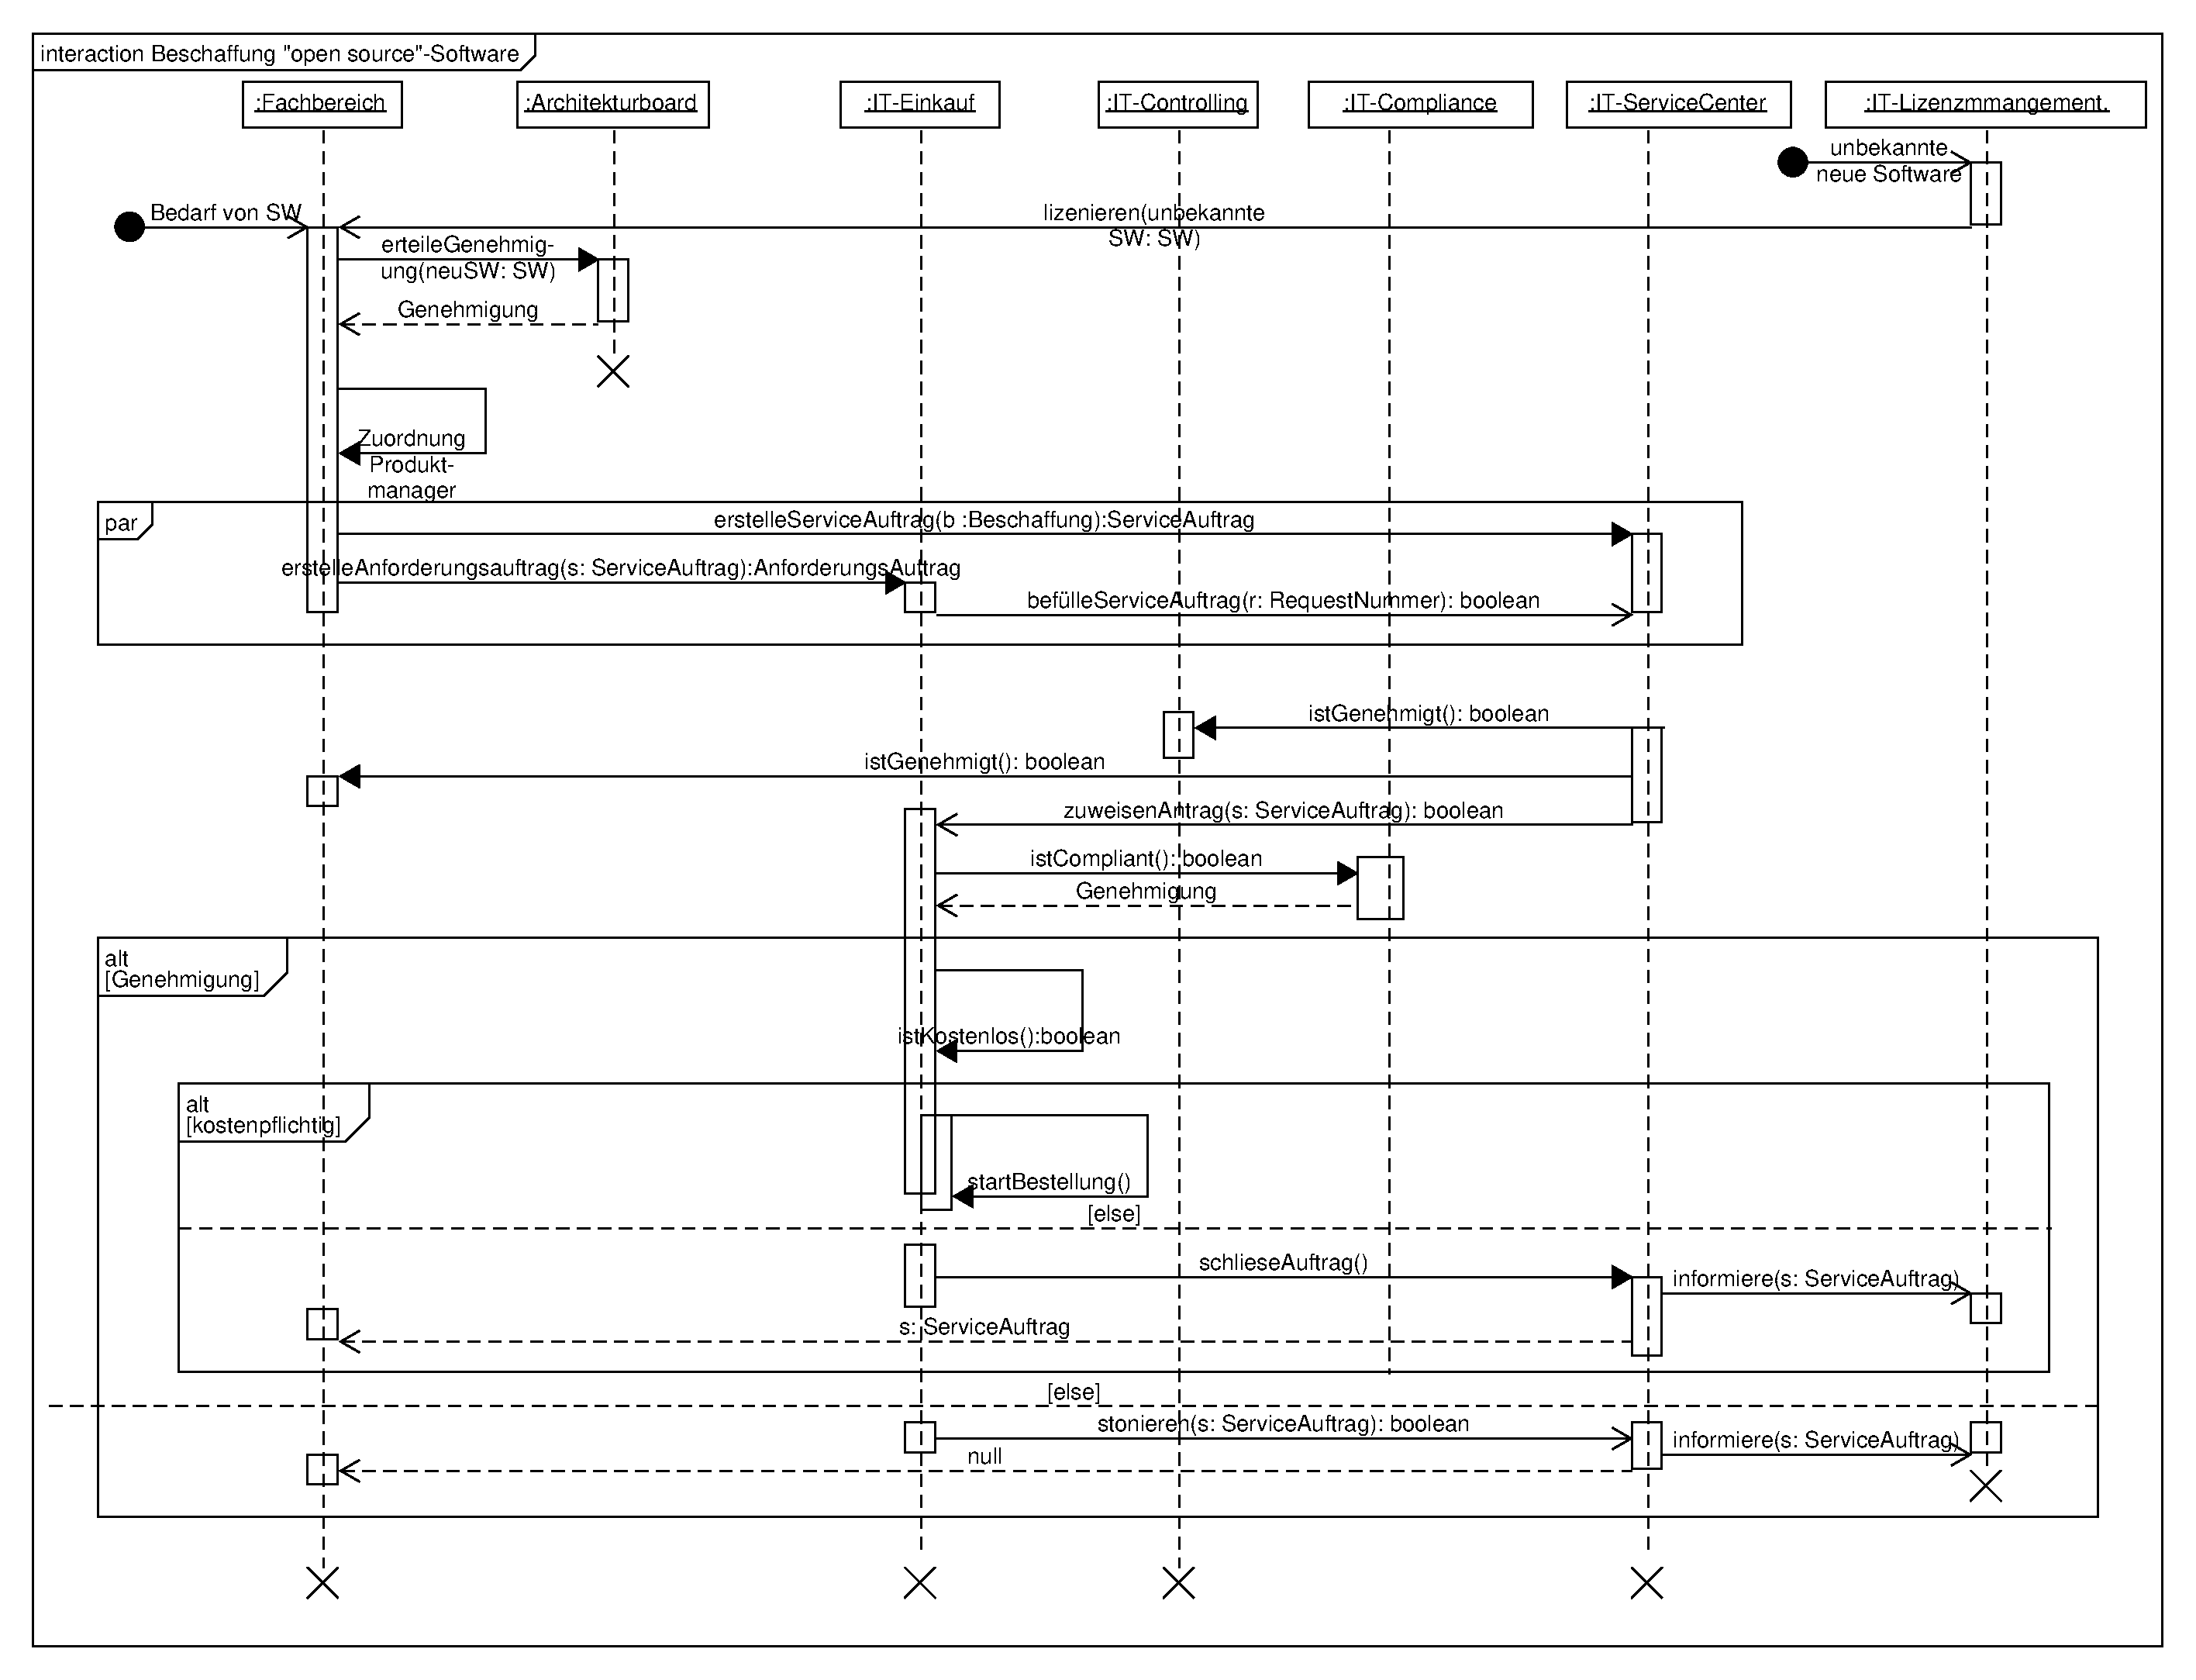
\includegraphics[scale=0.32]{img/prozessFreewareBeschaffung.pdf}
	\caption{(Adaptiertes) Sequenzdiagramm zur Beschaffung von \enquote{Open source}-Software}
	{\footnotesize Quelle: in Anlehnung an unternehmensinterne Prozessdokumentation \par \textit{unternehmensintern}}
	\label{abb:pFW}
\end{figure}

Die oben genannten Anforderungen erfüllen aus der Sicht der IT-Abteilung nicht die Kosten-Nutzen-Konformität. Aus rechtlicher Sicht ist das jedoch ein sehr hoch zu bewertendes Risiko, da es zu unmittelbaren juristischen Konsequenzen führen kann. Deswegen nutzt die IT-Abteilung meist den rechtlichen Prozess (juristische Prüfung von Vertragsdokumenten oder Sachverhalten), da dieser nicht die oben genannten Hürden enthält. Bei diesem wird der Verwendungszweck der Software erfragt und die geltenden Lizenzbedingungen durch \ac{IU11} geprüft. Jedoch ist davon auszugehen, dass eine offizielle Beschaffungsanfrage bei \enquote{Open source}-Software nur in wenigen\footnote{$ n \leq 10, n \in \mathbb{N}_{0} $, gemessen p. a.} Fällen gestellt wird. Begründet durch die Administrator-Berechtigung, die es Benutzern technisch erlaubt, auch ohne Restriktionen alles auf ihrem Computer zu installieren, kann keine numerische Aussage über die Dunkelziffer getroffen werden. Es bleibt nur die Hypothese der IT-Juristen der Abteilung \ac{IU11}, die weder falsifizierbar noch validierbar ist. 
\par
Ist die Software in der \ac{AWL} implementiert, gibt es noch eine Anwendung, \textsc{Nexus Lifecycle} von \textsc{sonatype}, die auf eventuelle Schwachstellen dieser benutzten Software prüft. \textsc{Nexus Lifecycle} ist eine Hilfsanwendung, die u. a. auch von \textsc{Creditreform} verwendet wird. Das Ziel dieses Produktes ist es, die gesamte Software-\enquote{Supply Chain} kontinuierlich zu bereinigen und sicher zu halten.\autocite[vgl.][]{sonatype_inc_nexus_2020} Aus dem Prüfbericht werden dann entsprechende Maßnahmen abgeleitet. Die erste ist die Software, in der die Schwachstelle gefunden wurde, als unsicher zu markieren und danach zu sperren. Die Entwicklungsabteilung muss versuchen, die Schwachstellen zu beseitigen. Problematisch ist es, wenn diese ignoriert werden. In letzter Konsequenz können der Betrieb und die Verteilung der Anwendung gestoppt werden. Dies führt zu massiven Problemen in der Produktion und somit verringert sich die vertragliche, mit dem Kunden vereinbarte, Verfügbarkeit der Systeme.

\section{Soll-Ist-Vergleich des in Forschungsfrage eins entworfenen Prozesses}
Die Abbildung \vref{abb:aufbauServerUmgebung} stellt den stark vereinfachten Aufbau der \textsc{OpenShift}-Umgebung im Rechenzentrum dar. Der Fokus liegt auf den einzelnen Komponenten. Diese können mittels eines Soll-Ist-Vergleichs zwischen den Anforderungen des Grundschutzes und den umgesetzten Vorkehrungen auf ihre Sicherheit überprüft werden. Dazu soll diese Abbildung \vref{abb:aufbauServerUmgebung} eine Übersicht der beteiligten Komponenten illustrieren. 

\begin{figure}[h!]
	\centering
	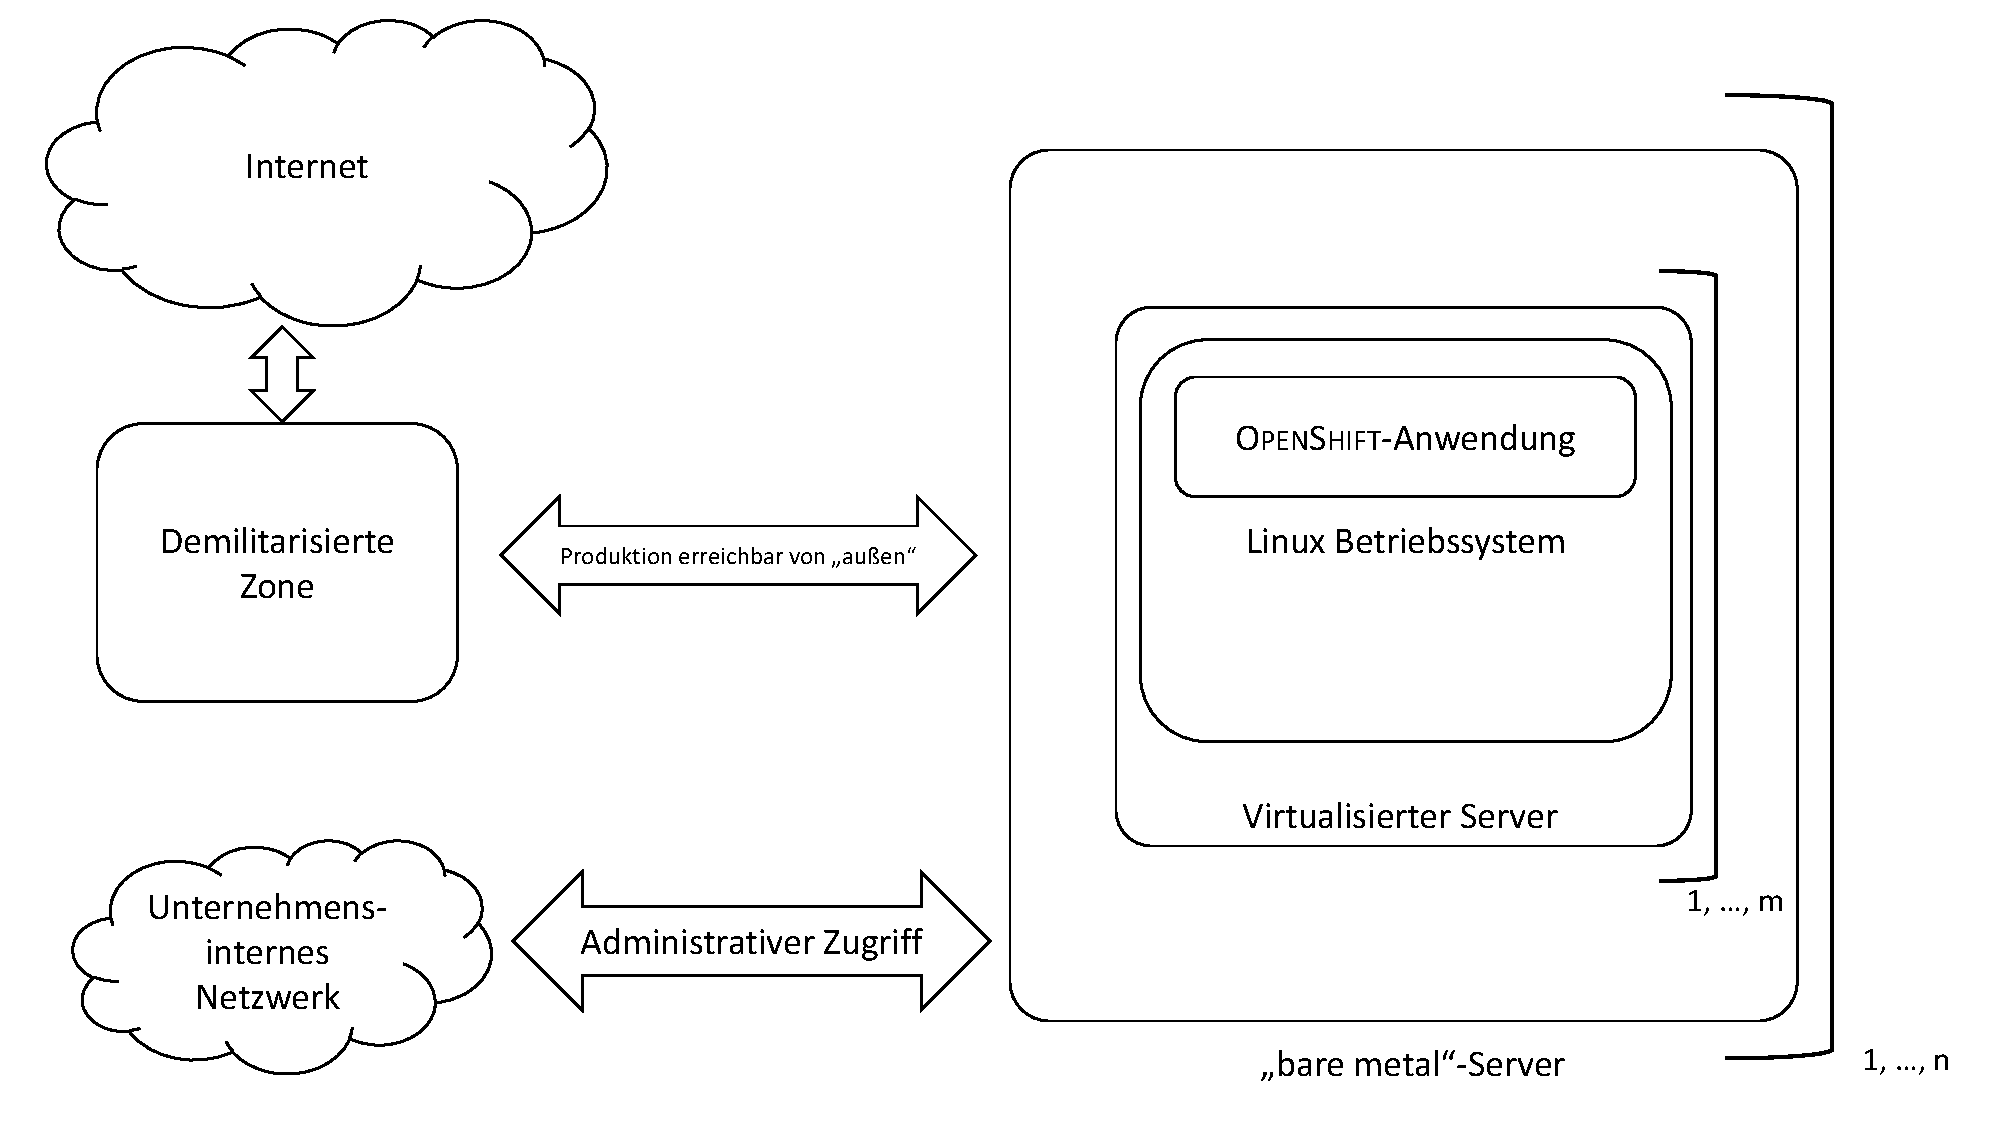
\includegraphics[scale=0.45]{img/aufbauOpenShiftServerUmgebung.pdf}
	\caption{Aufbau der \textsc{OpenShift}-Umgebung im Rechenzentrum}
	\label{abb:aufbauServerUmgebung}
	{\footnotesize Quelle: in Anlehnung an unternehmensinterne Dokumentation\par}
	{\footnotesize \textit{unternehmensintern}}
\end{figure}

Es werden folgende Komponenten identifiziert, die einer näheren Betrachtung und Bewertung durch das IT-Grundschutz-Kompendium des \ac{BSI} bedürfen: der \enquote{bare metal}-Server, der virtualisierte Server, das \textsc{Linux}-basierte Betriebssystem, die \textsc{OpenShift}-Anwendung, das Netzwerk beziehungsweise die demilitarisierte Zone\footnote{Anmerkung: Im Sinne der Informatik.} und das Rechenzentrum (der Vollständigkeit geschuldet). Die Bausteine (\enquote{Prozess-Bausteine}) werden mit Abkürzungen beschrieben.\autocite[vgl.][S.\,2-4]{bundesamt_fur_sicherheit_in_der_informationstechnik_bsi_it-grundschutz-kompendium_2020}\footnote{Außerdem ist das Schichtenmodell im Anhang \vref{abb:BSISchichtenmodell} dargestellt.} Die nachfolgende Betrachtung ist lediglich ein Überblick und müsste für eine Zertifizierung nach ISO 27001 detailreicher durchgeführt werden.
\par
Die Zuordnung der identifizierten Komponenten zu den Bausteinen des Grundschutzes ist der nächste wichtige Schritt, um den Soll-Ist-Vergleich durchzuführen. Die Tabelle \vref{tab:zuordnungKompBau} beschreibt diese Zuordnung. Im weiteren Verlauf wird die Kurzform der Komponenten-Baustein-Zuordnung mit der mathematisch korrekten Schreibweise $ Komponente\ k \mapsto Baustein\ b $ dargestellt.
\par

\begin{longtable}{@{}lp{8.0cm}@{}}
	\toprule[1.5pt]
	\textbf{Komponente} & \textbf{Bausteine des IT-Grundschutzes} \\* \midrule
	\endfirsthead
	%
	\multicolumn{2}{c}%
	{{\bfseries Tabelle \thetable\ von vorheriger Seite fortgeführt.}} \\
	\toprule
	\textbf{Komponente} & \textbf{Bausteine des IT-Grundschutzes} \\* \midrule
	\endhead
	%
	\bottomrule
	\endfoot
	%
	\endlastfoot
	%
	% below rules with content
	\enquote{Bare metal}-Server & SYS.1.1 Server\\
	Virtualisierte Server & SYS.1.5 Virtualisierung \\
	\textsc{Linux}-basierte Betriebssystem & SYS.1.3 Server unter Linux und Unix\\
	\textsc{OpenShift}-Anwendung & APP.3.1 Web-Anwendungen\\
	\pagebreak
	Netzwerk bzw. demilitarisierte Zone & NET.1 Netze und NET.3.2 \enquote{Firewall}\\
	Rechenzentrum & INF.2 Rechenzentrum sowie Serverräume\\* 
	
	\bottomrule[1.5pt]
	
	\caption{Zuordnung der Komponenten zu den Bausteinen}\label{tab:zuordnungKompBau}\\
\end{longtable}

Das \ac{ISMS} ist in der \ac{SVI} über den IT-Grundschutz implementiert. Die \ac{SV} verfügt über hochsensible, persönliche Kundendaten, wie z.\,B. Gesundheitsdaten. Diese sind hoch schutzbedürftig, da der Verlust, die Offenlegung oder die Verbreitung ein Vergehen nach dem Strafgesetzbuch\footnote{Das sind die einzigen Daten, die bei nicht-rechtskonformer Nutzung eine Freiheitsstrafe auslösen können.} darstellt. Für die Bereiche, in denen mit diesen Daten gearbeitet wird, konnten die vorgefertigten Bausteine nicht benutzt werden. Diese Bereiche sind einer vollumfänglichen Risikoanalyse nach dem ISO-Standard 27001 unterzogen worden. Da die Anwendung \textsc{Camunda}, für die der \enquote{Deployment}-Prozess initial erstellt wurde, keine Gesundheitsdaten verarbeiten wird, ist die Verwendung der Bausteine des \ac{BSI} laut der Empfehlung des \ac{BSI} ausreichend. Jedoch ist der \enquote{Deployment}-Prozess generisch angelegt und kann auch andere Container-Anwendungen verteilen. Die vorliegende Analyse bezieht sich dennoch auf eine Umgebung, die mittleren Schutzes bedarf, d.\,h., die Bausteine können verwendet werden. Dies ist begründet durch die Aussage der \enquote{Enterprise}-Architekten, dass ein Umzug der Bestandsführungssysteme (sie enthalten die hochsensiblen Daten) in Container-Anwendungen in den nächsten fünf Jahren nicht geplant sei. 
\par
\textbf{Komponente \enquote{Bare metal}-Server}:\label{sec:bareMetalServer}
\par
Diese wird dem Baustein \textit{SYS.1.1 Server} zu geordnet. Per Definition des \ac{BSI} ist ein allgemeiner Server folgendes Konstrukt: \enquote{[...] werden IT-Systeme mit einem beliebigen Betriebssystem bezeichnet, die Benutzern und anderen IT-Systemen Dienste bereitstellen. Diese Dienste können Basisdienste für das lokale oder externe Netz sein, aber auch den E-Mail-Austausch ermöglichen oder Datenbanken und Druckerdienste anbieten.}\autocite[][S.\,461]{bundesamt_fur_sicherheit_in_der_informationstechnik_bsi_it-grundschutz-kompendium_2020} Die identifizierte Gefährdungslage der \ac{BSI} sind Software-Schwachstellen und -Fehler, Datenverlust, \enquote{Denial of Service}-Angriffe, Überlastung der Server und Bereitstellung unnötiger Komponenten und Applikationen.\autocite[vgl.][S.\,461-462]{bundesamt_fur_sicherheit_in_der_informationstechnik_bsi_it-grundschutz-kompendium_2020} Diese Bedrohungen sind von der \ac{SVI} und der Rechenzentrumsbetreiberin erkannt. Diese Betreiberin steht in der Verantwortung, die Anforderungen des \ac{BSI} umzusetzen, da die \ac{SVI} das Rechenzentrumsmanagement an eine Dienstleisterin übergeben hat. Somit muss diese die Anforderungen implementieren. Jedoch kontrolliert die \ac{SVI} gemeinsam mit der \ac{SV} die Betreiberin durch ein internes jährliches Audit. Dies ist im Rahmenvertrag mit dem Unternehmen \textsc{Cancom} vereinbart. Auch der ständige Informationsaustausch ist eine Rahmenbedingung des Vertrages. Durch die Abtretung der Umsetzungsverantwortung begründet wird dieser Baustein durch diese Arbeit nicht näher beleuchtet. Die Maßnahmen des \ac{BSI} sind laut Geschäftsführung vollumfänglich implementiert.
\par
\textbf{Komponente Virtualisierte Server}:
\par
Für die Bewertung dieser Server wird laut \ac{BSI} folgender Baustein benutzt: $VServer \mapsto SYS.1.5\ Virtualisierung$. Die \ac{BSI} definiert: \enquote{Bei der Virtualisierung von IT-Systemen werden ein oder mehrere virtuelle IT-Systeme auf einem physischen IT-System ausgeführt. Ein solches physisches IT-System wird als „Virtualisierungsserver“ [sic!] bezeichnet. Mehrere Virtualisierungsserver können zu einer virtuellen Infrastruktur zusammengefasst werden. Darin können die Virtualisierungsserver selbst und die auf ihnen betriebenen virtuellen IT-Systeme gemeinsam verwaltet werden.}\autocite[][S.\,485]{bundesamt_fur_sicherheit_in_der_informationstechnik_bsi_it-grundschutz-kompendium_2020} Die identifizierten Gefährdungslagen sind fehlerhafte Planung oder Konfiguration der Virtualisierung, unzureichende Ressourcen für die IT-Systeme, Informationsabfluss oder Ressourcenengpass durch \enquote{snapshots}\footnote{Speicherung eins gewissen (vollumfänglichen) Zustands der virtuellen Maschine.}, Ausfall des Verwaltungsservers, missbräuchliche Nutzung von sogenannten Gastwerkzeugen\footnote{Damit können Laufwerke, Funktionen und Programme auf dem Gastsystem eingespielt werden.} und die Kompromittierung der Virtualisierungssoftware.\autocite[vgl.][S.\,486-487]{bundesamt_fur_sicherheit_in_der_informationstechnik_bsi_it-grundschutz-kompendium_2020} Diese Server unterliegen auch dem Management der Dienstleisterin der \ac{SVI}. Deswegen ist die Begründung die gleiche, wie in Kapitel \vref{sec:bareMetalServer} Absatz \enquote{Komponente \enquote{Bare metal}-Server}. 
\par
\textbf{Komponente \textsc{Linux}\footnote{Formal nicht korrekt, da es \textsc{Unix}- und \textsc{Linux}-Systeme gibt. Hier wird \textsc{Linux} als Sammelbegriff für beide Gattung verwendet.}-basierte Betriebssysteme}:
\par
Diese können durch die Anforderungen des Bausteins \textit{SYS.1.3 Server unter Linux und Unix} abgesichert werden. Die Definition des \textit{SYS.1.3} lautet: \enquote{Auf Server-Systemen werden häufig die Betriebssysteme Linux oder Unix eingesetzt. Beispiele für klassische UnixSysteme [sic!] sind die BSD-Reihe (FreeBSD, OpenBSD und NetBSD), Solaris und AIX. Linux bezeichnet hingegen kein klassisches Unix, sondern ist ein funktionelles Unix-System. Das heißt, dass der Linux-Kernel nicht auf dem ursprünglichen Quelltext basiert, aus dem sich die verschiedenen Unix-Derivate entwickelt haben. In diesem Baustein werden alle Betriebssysteme der Unix-Familie betrachtet, also auch Linux als funktionelles Unix-System. Da sich die	Konfiguration und der Betrieb von Linux- und Unix-Servern ähneln, werden in diesem Baustein Linux und Unix sprachlich als „Unix-Server“ bzw. „unixartig“ zusammengefasst.}\autocite[][S.\,480]{bundesamt_fur_sicherheit_in_der_informationstechnik_bsi_it-grundschutz-kompendium_2020} Die Gefährdungslagen sind ausspähen von System- und Benutzerinformationen, Ausnutzbarkeit der Skript-Umgebung, dynamisches Laden von gemeinsam genutzten Bibliotheken und Software aus Drittquellen.\autocite[vgl.][S.\,480]{bundesamt_fur_sicherheit_in_der_informationstechnik_bsi_it-grundschutz-kompendium_2020} Diese Systeme sind in der vollständigen Verantwortung der \ac{SVI} und müssen deswegen durch die Implementierung von Sicherheitsmaßnahmen geschützt werden. Das \ac{BSI} definiert die grundsätzliche Zuständigkeit für die Systeme als Abteilung Betrieb. Des Weiteren sind folgende Anforderungen an diese IT-Systeme beschrieben: Authentisierung von Administratorinnen und Benutzerinnen, sorgfältige Vergabe von Benutzerinnenkennungen, kein automatisches Einbinden von Wechsellaufwerken, Schutz vor Ausnutzung von Schwachstellen in Anwendungen, sichere Installation von Software-Paketen, zentrale Verwaltung von Benutzerinnen und Gruppen, verschlüsselter Zugriff auf die Skript-Umgebung, Absicherung des Startvorgangs, der Einsatz von Sicherungsmaßnahmen des Dateisystems, zusätzlicher Schutz bei erhöhtem Sicherheitsbedarf (abgekürzt, da nicht relevant für die \textsc{Linux}-Systeme der \ac{SVI})\autocite[vgl.][S.\,480-482]{bundesamt_fur_sicherheit_in_der_informationstechnik_bsi_it-grundschutz-kompendium_2020}. Die \ac{SVI} setzt viele der oben genannten Maßnahmen um. Die Authentifizierung von Administratorinnen und Benutzerinnen erfolgt durch die Anmeldung an dem Server. Benutzerinnenkonten müssen immer über einen internen Beauftragungsprozess beantragt werden. Dadurch kann keine Benutzerin ihre Rechte auf einem System ohne Freigabe ändern bzw. erweitern. Bei der Beauftragung müssen alle zusätzlichen Privilegien begründet werden, z.\,B. das Recht ein Skript oder ein Programm als Administratorin auszuführen. Jedes Benutzerinnenkonto ist personalisiert anzulegen, da somit die Nachverfolgbarkeit gewährleistet ist. Technische Benutzerinnen sind auf den IT-Systemen abzuschaffen und durch personalisierte Versionen zu ersetzen. Diese Anforderung begründet die \ac{SVI} durch die Sicherheitsvorschriften. Durch den Prozess wird auch eine übermäßige, unkontrollierte Ausgabe von Konten auf einem System verhindert, so ist zu jedem Zeitpunkt bekannt, welche Personen Zugriff auf das System mit welchen Rechten haben. Wechsellaufwerke können auf den Systemen nicht eingebunden werden. Die Kernel der Systeme der \ac{SVI} den für die Finanzdienstleistung vorgeschrieben Regularien geschützt, so ist die Verwendung von Drittanbieterinen-Anwendungen nicht möglich. Auch sind alle Sicherheits-\enquote{updates} einzuspielen. Die Installation von Software erfolgt bei der \ac{SVI} nicht durch die Benutzerin der Anwendung, sondern sie beauftragt die Installation mittels \enquote{Service request}. Dieser Prozess implementiert Sicherheitsvorkehrungen. So ist die Installation immer von mindestens einer anderen nicht beteiligten Person kontrolliert. Die Dateien und Zustände der Systeme werden durch einen ständigen Zyklus gesichert. Diese Datensicherung ist unabhängig von der \ac{AWL} betrieben, d.\,h. bei einem Virusbefall sind die Sicherungen physisch nicht-erreichbar und somit geschützt. Wichtig ist es, dass die Maßnahmen ständig auf ihre Wirksamkeit überprüft werden. Die \ac{SVI} hat dazu interne Sicherheits-Audits implementiert, die im sechsmonatigem Rhythmus überprüfen, ob alle Sicherheitsstandards eingehalten werden. Die Betriebsabteilungen sind angehalten Sicherheits-\enquote{updates} direkt nach Bekanntgabe der Herstellerinnen solche in die Systeme einzuspielen.
\par
\textbf{Komponente \textsc{OpenShift}-Anwendung}:
\par
Diese Komponente wird durch die Anforderungen des Bausteins \textit{APP.3.1 Web-Anwen-dungen} teilweise beschrieben. Die Einschränkung bezieht sich auf die Nutzung des Kunden über eine Webanbindung mittels des Protokolls \ac{HTTPS}. Die Absicherung der Webdienste wird nachfolgend betrachet. Die Definition des Begriffes \textit{APP.3.1} lautet: \enquote{Webanwendungen stellen Funktionen und dynamische Inhalte zur Verfügung. Sie nutzen dazu das Internetprotokoll HTTP (Hypertext Transfer Protocol) bzw. HTTPS. Bei HTTPS wird die Verbindung durch die Protokolle SSL (Secure Socket Layer) oder TLS (Transport Layer Security) verschlüsselt und zusätzlich gesichert. Webanwendungen erstellen auf einem Server Dokumente und Benutzeroberflächen, z. B. Eingabemasken, und liefern diese an entsprechende Clientprogramme, wie etwa Webbrowser. Webanwendungen werden gewöhnlich auf der Grundlage von Frameworks entwickelt. Diese stellen ein Rahmenwerk für häufig wiederkehrende Aufgaben zur Verfügung, z.\,B. für Sicherheitskomponenten.}\autocite[][S.\,383]{bundesamt_fur_sicherheit_in_der_informationstechnik_bsi_it-grundschutz-kompendium_2020} Die Sicherheit wird durch Anforderungen des \ac{BSI} umgesetzt, diese sind: Authentifizierung der Entwicklerinnen, Zugriffskontrolle, Protokollierung sicherheitsrelevanter Ereignisse, Schutz vor unerlaubter Nutzung, Schutz von vertraulichen Daten, Architekturanforderungen, sichere Anbindung von Hintergrundsystemen und Konfiguration der Webanwendung.\autocite[vgl.][S.\,385-389]{bundesamt_fur_sicherheit_in_der_informationstechnik_bsi_it-grundschutz-kompendium_2020} Der Baustein \textit{APP.3.1} ist initial nicht für eine \enquote{Cloud}-Anwendung, wie es \textsc{OpenShift} ist, bestimmt. Das \ac{BSI} beschreibt in diesem Baustein den Webserver, der \textsc{HTML}- oder \textsc{PHP}-Seiten darstellt. Jedoch bietet die \ac{BSI} die Baustein \textit{OPS.2.2 Cloud-Nutzung} an, der sich auf die allgemeine Nutzung von \enquote{Cloud}-Diensten bezieht. Dieser definiert \enquote{Cloud Computing bezeichnet das dynamisch an den Bedarf angepasste Anbieten, Nutzen und Abrechnen von IT-Dienstleistungen über ein Netz. Angebot und Nutzung dieser Dienstleistungen erfolgen dabei ausschließlich über definierte technische Schnittstellen und Protokolle. Die Spannbreite der im Rahmen von Cloud Computing angebotenen Dienstleistungen umfasst das komplette Spektrum der Informationstechnik und beinhaltet unter anderem Infrastruktur (z. B. Rechenleistung, Speicherplatz), Plattformen und Software.}\autocite[][S.\,265]{bundesamt_fur_sicherheit_in_der_informationstechnik_bsi_it-grundschutz-kompendium_2020} Dieser Baustein spiegelt den Vorteil der Plattform \textsc{OpenShift} wieder, die Anwendungen an dynamisch skaliert. Die Sicherheitsvorkehrungen dieses Bausteines sind die Erstellung einer \enquote{Cloud}-Nutzungsstrategie und von Sicherheitsrichtlinien, die Festlegung von Verantwortlichkeiten und Schnittstellen, die Erstellung eines Notfallkonzepts und Bedingungen, die einen Ausstieg der \enquote{Cloud}-Nutzung ermöglichen.\autocite[vgl.][S.\,268-271]{bundesamt_fur_sicherheit_in_der_informationstechnik_bsi_it-grundschutz-kompendium_2020} Die \ac{SVI} betreibt die \enquote{OpenShift}- und damit die \enquote{Cloud}-Umgebung im  eigenen Rechenzentrum, dass von ihrer Dienstleisterin betrieben wird. Jedoch ist die \ac{SVI} für die Sicherung der Anwendungen selbst verantwortlich. Die Nutzungsstrategie beschränkt sich zum Zeitpunkt der Erstellung der Arbeit auf die Verprobung der Anwendung \textsc{Camunda} in einer Labor-Umgebung. Die Nutzungsstrategie für das Produktivsystem wird von den \enquote{Enterprise}-Architekten in Zusammenarbeit mit der IT-Sicherheitsabteilung ausgearbeitet. Die Verantwortlichkeiten sind strikt aufgeteilt: die Betriebsabteilung kümmert sich um das Management und die administrativen Aufgaben; die Abteilung \ac{IE2} entwickelt, betreibt, prüft und dokumentiert die \enquote{Deployments} und die Entwicklungsabteilungen bzw. -teams erstellen die Container-Anwendungen zur Übergabe an \ac{IE2}. Die initialen Sicherheitsrichtlinien sind von den Entwicklungsrichtlinien abgeleitet. Diese schreiben beispielsweise vor bei Webanwendungen alle \enquote{Ports} zu blocken bis auf die notwendigen \enquote{Ports}. Die Schnittstellen werden in drei ausgeteilt: Übergabe der entwickelten Anwendung an \ac{IE2} durch die Entwicklungsabteilungen, die Beauftragung von administrativen Aufgaben durch, erstens, die Entwicklungsteams oder, zweitens, durch die Abteilung \ac{IE2}. Das Notfallkonzept schreibt u. a. vor, dass die \textsc{OpenShift}-Umgebung ein vollständiges Parallel-System haben muss, dass im Notfall einspringt. Dies wurde bei der Kaufentscheidung berücksichtigt. Der Ausstieg aus Systemen wird in der \ac{SVI} bei eigenem Betrieb im Rechenzentrum nur geplant, wenn die Anforderung der Ablösung besteht.
\par
\textbf{Komponente Netzwerk bzw. demilitarisierte Zone}:
\par
Die Sicherheit dieses Bausteins wird durch die Anforderung des \textit{NET.1 Netze und NET.3.2 \enquote{Firewall}} beschrieben. Die Definition des Begriffs \textit{NET.1} lautet: \enquote{Die meisten Institutionen benötigen heute für ihren Geschäftsbetrieb und für die Erfüllung ihrer Fachaufgaben Datennetze, über die beispielsweise Informationen und Daten ausgetauscht sowie verteilte Anwendungen realisiert	werden. In solche Netze werden nicht nur herkömmliche Endgeräte, Partner-Institutionen und das Internet angeschlossen. Sie integrieren zunehmend auch mobile Endgeräte und Elemente, die dem Internet of Things (IoT) zugerechnet werden. Darüber hinaus werden über Datennetze vermehrt auch Cloud-Dienste sowie Dienste für Unified	Communication and Collaboration (UCC) [sic!] genutzt. Die Vorteile, die sich dadurch ergeben, sind unbestritten.}\autocite[][S.\,669]{bundesamt_fur_sicherheit_in_der_informationstechnik_bsi_it-grundschutz-kompendium_2020} Die \enquote{Firewall} beschreibt die \ac{BSI} so: \enquote{Eine Firewall ist ein System aus soft- und hardwaretechnischen [sic!] Komponenten, das dazu eingesetzt wird, IP-basierte Datennetze sicher zu koppeln. Dazu wird mithilfe einer Firewall-Struktur der technisch mögliche Informationsfluss auf die in einer Sicherheitsrichtlinie als vorher sicher definierte Kommunikation eingeschränkt. Sicher bedeutet hierbei, dass ausschließlich die erwünschten Zugriffe oder Datenströme zwischen verschiedenen Netzen zugelassen werden.}\autocite[][S.\,711]{bundesamt_fur_sicherheit_in_der_informationstechnik_bsi_it-grundschutz-kompendium_2020} Das Netzwerk und die demilitarisierte Zone befinden sich, wie auch die Server-Komponenten und nachfolgend das Rechenzentrum, in der vollumfänglichen Verantwortung \ac{SVI}-Dienstleisterin. Die Regelungen des Rahmenvertrages gelten auch hier. Die Audits aus den Jahren 2018 und 2019 haben ergeben, dass es keine relevanten Sicherheitsvorfälle gab und das vereinbarte Sicherheitslevel zu jedem Zeitpunkt eingehalten war. 
\par
\textbf{Komponente Rechenzentrum}:
\par
Diese ist durch den Baustein \textit{INF.2 Rechenzentrum sowie Serverräume} beschrieben. Die eine Definition des \ac{BSI} lautet: \enquote{Wird die IT der Institution innerhalb eines Gebäudes oder einer Liegenschaft verteilt in mehreren Bereichen betrieben und sind diese Bereiche untereinander und zu den IT-Benutzern hin durch hauseigene LAN-Verbindungen angeschlossen, ist mindestens der funktional bedeutendste dieser Bereiche als RZ zu behandeln. Des Weiteren sind Bereiche, von deren ordnungsgemäßem Betrieb 50\,\% und mehr Nutzer abhängig sind oder aus denen heraus 50\,\% und mehr an Diensten und Daten (gemessen an der Gesamtheit der Bereiche) bereitgestellt werden, als RZ zu behandeln.}\autocite[][S.\,755]{bundesamt_fur_sicherheit_in_der_informationstechnik_bsi_it-grundschutz-kompendium_2020} Diese Definition trifft auf die Lage des Rechenzentrums der \ac{SVI} zu, denn sie ist an zwei Orten im Stuttgarter Raum verteilt und besteht aus einer Serverlandschaft. Der Betrieb, die Wartung und das Management (zu großen Teilen) werden durch die Dienstleisterin der \ac{SVI} durchgeführt. Die Verantwortung der Erfüllung aller sicherheitsrelevanter Bestimmungen und Maßnahmen obliegt der Betreiberin. Diese sind in einem Rahmenvertrag vereinbart. Begründet durch diese Tatsache sieht diese Arbeit von der weiteren Betrachtung der Komponente Rechenzentrum ab.

\section{Ergebnis der Forschungsfrage drei}
Abschließend ist hervorzuheben, dass dieses Kapitel einen Überblick über die Sicherheitskonzepte der \ac{SVI} darstellt. Eine vollständige Risikoanalyse übersteigt den Umfang dieser Arbeit, da der Fokus der Arbeit auf der Forschungsfrage eins (Kapitel \vref{ff1}) liegt. 

\paragraph{Abschließende Sicherheitsprüfung} Die Sicherheitsprüfung bzw. der Vergleich ist nicht abgeschlossen und genügt den Anforderungen nicht, die im Grundlagenteil dieses Kapitels (vgl. Kapitel \vref{kap:sicherheitstechnischeAnforderungen}) beschrieben werden. Dies ist dem Umstand geschuldet, dass alle relevanten Sicherheitsvorkehrungen durch die \ac{SVI} und ihre Dienstleisterinnen implementiert sind. Dies ist eine zwingende Anforderung der \ac{SVI} bevor ein System (Anwendungen, Server o.\,Ä.) produktiv geht. Die abschließende Entwicklung eines Sicherheitskonzeptes muss vor dem Produktivgang der \textsc{OpenShift}-Anwendung nochmals überprüft und in Zusammenarbeit mit den IT-Dienstleisterinnen der \ac{SVI} verbessert werden. Kritisch zu betrachten ist, dass der Soll-Ist-Vergleich nicht tiefgreifende Informationen generiert hat. 

\paragraph{Einschränkungen durch den Labor-Betrieb} Der Labor-Betrieb der \textsc{OpenShift}-Umgebung schränkt die Risikoanalyse ein, da in einem abgeschlossenen Labor in der \ac{SVI} die Anwendungs-spezifischen Sicherheitsvorkehrungen nicht implementiert werden, die dieses Labor keinen Zugang zur produktiven \ac{AWL} besitzt. Netzwerk-technisch wie auch physikalisch sind Labor-Umgebung vollständig von der \ac{AWL} getrennt. Aus diesem Grund genügt der Soll-Ist-Vergleich der Labor-Umgebung und muss nochmals für die produktiven Systeme ausgeführt werden.

\paragraph{Ausblick} Falls die Geschäftsführung sich entscheidet auch die Bestandssysteme in Container-Anwendungen zu verlagern, erhöhen sich die sicherheitsrelevanten Anforderungen, da Gesundheitsdaten der Kunden der \ac{SV} in den Containern verarbeitet werden. Dadurch müssen die Sicherheitsvorkehrungen ausgeweitet werden, um die \enquote{Cloud}-Plattform \textsc{OpenShift} weiter zu schützen. Bei produktiven Systemen reicht das hier dargestellte Vorgehen nicht aus, es müssten bei allen Komponenten eigene Risikoanalysen durchgeführt werden und es würde die Verwendung der \ac{BSI}-Bausteine nicht mehr ausreichend sein. In der produktiven \ac{AWL} werden sensible Daten verwaltet, die erhöhte Sicherheitsvorkehrungen nach der ISO-Norm 27001\autocite[vgl.][]{dindeutsches_institut_fur_normung_informationstechnik_2020} und der Empfehlung des \ac{BSI} im IT-Grundschutz\autocite[vgl.][]{bundesamt_fur_sicherheit_in_der_informationstechnik_bsi_it-grundschutz-kompendium_2020} benötigen. Eine weitere Risikobetrachtung durch die Teams der IT-\enquote{Compliance} des \ac{SVI} und der Riskobewertungsabteilung der \ac{SV} muss durchgeführt werden. 
